\section{The rolling tachyon and tachyon matter}\label{sec:rolling}

\subsection{Homogeneous decay}\label{ssec:homogeneous}

Sen \cite{Sen02rolling} described the time-dependent decay of an unstable D$p$-brane by the boundary conformal field theory with the marginal deformation $\lambda\int \cosh X^0$ of the free boson $X^0$ on the boundary of the world-sheet, and computed the energy-momentum tensor from the boundary state. In the bosonic string, for $0\le\lambda\le\frac12$,
\begin{equation}\label{eq:rolling}
\begin{gathered}
T_{00} = \tfrac{1}{2}\mathcal T_p\big(1+\cos 2\pi\lambda\big) ,\qquad
T_{ij} = -\delta_{ij}\,\mathcal T_p\,f(x^0),\\
f(x^0) = \frac{1}{1+e^{x^0}\sin\pi\lambda} + \frac{1}{1+e^{-x^0}\sin\pi\lambda} - 1 ,
\end{gathered}
\end{equation}
and in the superstring the same with $x^0$ replaced by $x^0/\sqrt2$ and $\sin\pi\lambda$ by $\sin^2\pi\lambda$.

\begin{theorem}[claim 16; Sen 2002]\label{thm:homogeneous}
The energy density \eqref{eq:rolling} is conserved, and the pressure $-\mathcal T_p f(x^0)$ tends to zero as $x^0\to\pm\infty$, as $e^{-|x^0|}$ in the bosonic string and $e^{-|x^0|/\sqrt2}$ in the superstring. For $\lambda=\frac12$ the energy density vanishes and the solution is the tachyon vacuum at all times.
\end{theorem}

\begin{proof}
The boundary state is the product of the Dirichlet boundary state for the spatial directions, the $c=1$ boundary state of the $\cosh X^0$ deformation, obtained by Wick rotation of the $SU(2)$ rotation of the Neumann boundary state at the self-dual radius, and the ghost boundary state; $T_{\mu\nu}$ is read off from the coefficient of the closed string graviton. As $x^0\to+\infty$ the first term of $f$ is $O(e^{-x^0})$ and the second is $1 - \sin\pi\lambda\, e^{-x^0} + O(e^{-2x^0})$, so $f = O(e^{-x^0})$; the case $x^0\to-\infty$ is symmetric. Conservation is $\partial_0 T_{00}=0$, immediate from the form of $T_{00}$. This is \cite[Section~3]{Sen02rolling}; the computation is exact in $\alpha'$ and at tree level in the string coupling.
\end{proof}

\begin{verdict}[claim 16]
Proved. The statement is a theorem of boundary conformal field theory. The open question is its physical scope, treated in Section~\ref{ssec:emission}.
\end{verdict}

\subsection{Tachyon matter and the caustic theorem}\label{ssec:caustic}

Sen \cite{Sen02matter} called the asymptotic state of \eqref{eq:rolling}, with constant energy density and vanishing pressure, \emph{tachyon matter}, and \cite{Sen02field} proposed an effective field theory for the tachyon near the minimum of its potential whose solutions are this matter:
\begin{equation}\label{eq:dbi}
\begin{gathered}
S = -\int d^{p+1}x\; V(T)\sqrt{1+\eta^{\mu\nu}\partial_\mu T\partial_\nu T},\\
\eta = \operatorname{diag}(-1,1,\dots,1),\qquad V(T)\to 0 \text{ as } T\to\infty .
\end{gathered}
\end{equation}
The abstract of \cite{Sen02matter} states the conclusion: \fatal{``in both cases the asymptotic form of the energy momentum tensor for large time is described by a pressureless gas with non-zero energy density''}, the two cases being the bosonic string and the superstring; and \cite{Sen02field} states that the classical solutions of \eqref{eq:dbi} near the minimum ``include non-relativistic matter with arbitrary spatial distribution of energy''. Both sentences are proved in \cite{Sen02rolling,Sen02matter} for spatially homogeneous decay, and the second is correct as a statement about the existence of solutions at one instant. Read as a statement about the end state of the decay of a brane whose tachyon is not homogeneous, which is how the two papers and much of the literature read it, the first sentence is false, and the reason is in the equations of \cite{Sen02field} themselves.

Near the minimum, $V\to0$, the equation of motion of \eqref{eq:dbi} forces $\eta^{\mu\nu}\partial_\mu T\partial_\nu T\to -1$ wherever the energy density stays finite \cite[Section~2]{Sen02field}, and the energy-momentum tensor takes the form
\begin{equation}\label{eq:dust}
T^{\mu\nu} = \rho\, u^\mu u^\nu,\qquad u^\mu = -\eta^{\mu\nu}\partial_\nu T,\qquad u^\mu u_\mu = -1,
\end{equation}
of a pressureless fluid with velocity $u^\mu$ and rest density $\rho = V(T)/\sqrt{1+\partial T\cdot\partial T}\ \ge 0$. We write $W = \partial_t T = \sqrt{1+|\nabla T|^2}$ for the branch in which $T$ increases with time (the other branch is obtained by $T\mapsto -T$), $v = -\nabla T/W$ for the three-velocity $u^i/u^0$ of the fluid, and $\eps = T^{00} = \rho W^2$ for the energy density.

\begin{lemma}\label{lem:dustflow}
Let $T$ be a $C^2$ solution of $\eta^{\mu\nu}\partial_\mu T\partial_\nu T = -1$ on $[0,t_1)\times\RR^p$ with $\partial_t T>0$, and let $\rho\ge0$ be $C^1$ with $\partial_\mu(\rho u^\mu) = 0$. Then:
\begin{enumerate}[label=(\roman*),leftmargin=2em]
\item $u^\mu\partial_\mu u^\nu = 0$: the integral curves of $u$, equivalently the curves $\dot X = v(t,X)$, are straight lines $X(t;x_0) = x_0 + t\,v_0(x_0)$, $v_0 = v(0,\cdot)$, along which $v$ is constant;
\item $\partial_t\eps + \partial_i(\eps v^i) = 0$, and along the lines of (i)
\[
\eps\big(t,X(t;x_0)\big)\det\big(I + t\,Dv_0(x_0)\big) = \eps(0,x_0);
\]
\item $Dv_0 = -W^{-1}P\,H$ with $H = \nabla^2 T(0,\cdot)$ the Hessian of the initial profile and $P = I - \nabla T\nabla T^{\mathsf T}/W^2$ symmetric and positive definite; the eigenvalues of $Dv_0(x_0)$ are real, and $Dv_0(x_0)$ has a negative eigenvalue if and only if $H(x_0)$ has one.
\end{enumerate}
\end{lemma}

\begin{proof}
(i) Since $u_\mu = -\partial_\mu T$ is a gradient,
\[
u^\mu\partial_\mu u_\nu = u^\mu\partial_\nu u_\mu = \tfrac12\partial_\nu(u^\mu u_\mu) = 0 .
\]
In components, with $u^0=W$ and $u^i = Wv^i$, the equations $u^\mu\partial_\mu W = 0$ and $u^\mu\partial_\mu(Wv^i)=0$ give $(\partial_t + v\cdot\nabla)v = 0$, so $v$ is constant along the curves $\dot X = v$, which are therefore straight. (ii) $\partial_\mu(\rho u^\mu u^0) = u^0\partial_\mu(\rho u^\mu) + \rho u^\mu\partial_\mu u^0 = 0$ is the continuity equation for $\eps = \rho W^2$ with flux $\eps v$. Writing it as $(\partial_t + v\cdot\nabla)\eps = -\eps\,\nabla\!\cdot v$ and using
\[
\nabla\!\cdot v\big(t,X(t;x_0)\big) = \tfrac{d}{dt}\ln\det\big(I+tDv_0(x_0)\big),
\]
which holds because the Jacobian $D_{x_0}X = I + tDv_0$ satisfies $\tfrac{d}{dt}D_{x_0}X = (Dv)(D_{x_0}X)$, gives
\[
\tfrac{d}{dt}\big[\eps\det(I+tDv_0)\big] = 0
\]
along the line. (iii) Differentiating $v^i = -\partial_iT/W$ and $W^2 = 1+|\nabla T|^2$ gives $\partial_j v^i = -W^{-1}\big(\delta_{ik} - \partial_iT\partial_kT/W^2\big)\partial_k\partial_jT$. The matrix $P$ has eigenvalue $1$ on the orthogonal complement of $\nabla T$ and $1-|\nabla T|^2/W^2 = W^{-2}>0$ along it. $PH$ is similar to $P^{1/2}HP^{1/2}$, which is symmetric, so its eigenvalues are real, and by Sylvester's law of inertia $P^{1/2}HP^{1/2}$ and $H$ have the same number of negative eigenvalues.
\end{proof}

\begin{theorem}[claim 17 fails as stated]\label{thm:caustic}
Let $T_0\in C^2(\RR^p)$ be the initial profile of a solution of the dust equations \eqref{eq:dust} of \cite{Sen02field}, on the branch $\partial_tT>0$, with initial energy density $\eps_0>0$. Let
\begin{equation}\label{eq:tc}
\begin{gathered}
\mu_- = \sup_{x_0\in\RR^p}\ \max\big\{-\lambda : \lambda \text{ an eigenvalue of } Dv_0(x_0)\big\} ,\\
Dv_0 = -\frac{P\,\nabla^2 T_0}{\sqrt{1+|\nabla T_0|^2}} .
\end{gathered}
\end{equation}
\begin{enumerate}[label=(\roman*),leftmargin=2em]
\item If $T_0$ is convex, $\mu_-\le 0$: along every characteristic the Jacobian $\det(I+tDv_0(x_0))$ is at least $1$ for all $t\ge0$, the energy density is non-increasing, and no caustic forms.
\item If $T_0$ is not convex, then $0<\mu_-\le\infty$ and the solution develops a caustic at the time $t_c = 1/\mu_-$: two characteristics meet, the Jacobian $\det(I+tDv_0)$ vanishes along some characteristic, and the energy density $\eps$ along that characteristic tends to $+\infty$ as $t\uparrow t_c$. The solution of the dust equations does not extend past $t_c$ as a single-valued field.
\item Every bounded non-constant $T_0$, in particular every periodic or compactly supported non-constant perturbation of the homogeneous decay, falls under (ii).
\item For $p=1$: $v_0' = -T_0''/(1+T_0'^2)^{3/2}$, the caustic forms if and only if $T_0''>0$ somewhere, $t_c = \big(\sup_x T_0''(x)/(1+T_0'(x)^2)^{3/2}\big)^{-1}$, and $\eps(t,X(t;x_0)) = \eps_0(x_0)/(1+t\,v_0'(x_0))$.
\end{enumerate}
\end{theorem}

\begin{figure}[t]
\centering
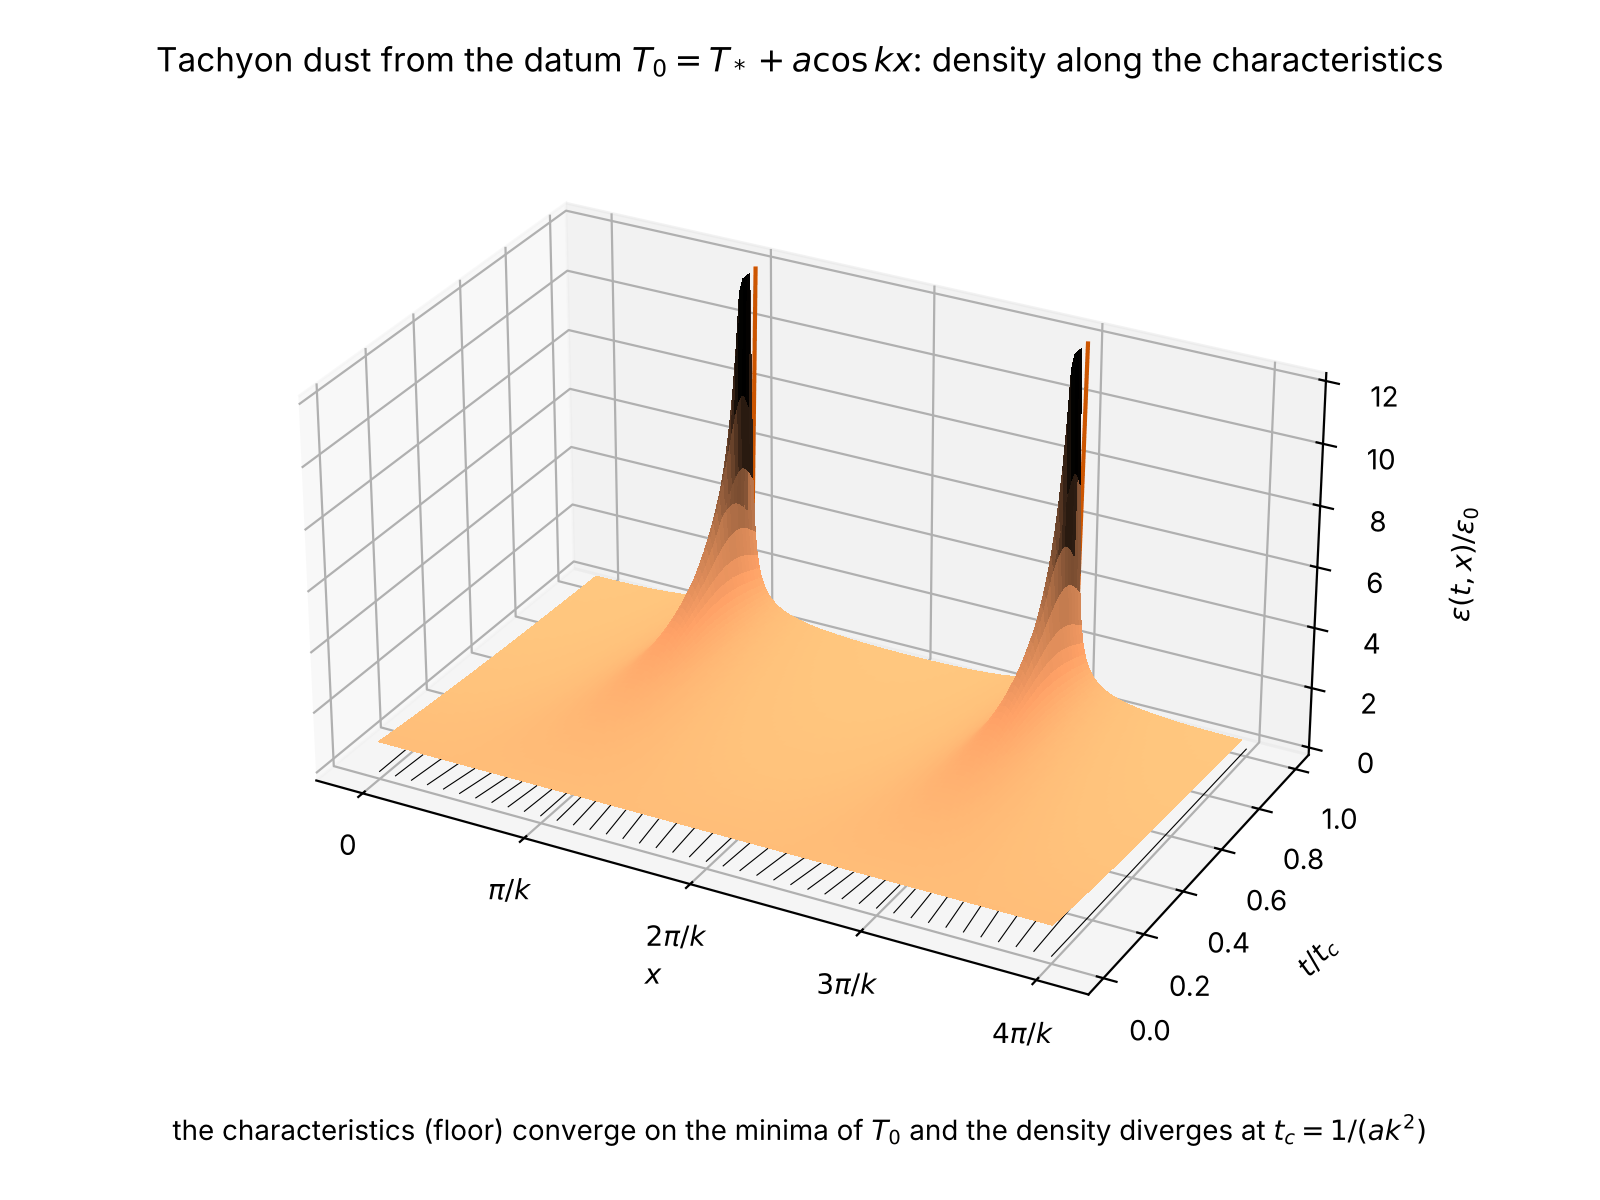
\includegraphics[width=\columnwidth]{figures/fig_caustic.png}
\caption{The dust of Theorem~\ref{thm:caustic} for the datum $T_0 = T_* + a\cos kx$ of Appendix~\ref{app:dust}, with $a = 1/2$, $k = 1$. The characteristics, drawn on the floor, are straight lines that converge on the minima of $T_0$; the energy density along them is $\eps_0/(1 + t\,v_0'(x_0))$ and diverges at $t_c = 1/(ak^2)$, where the vertical lines stand. The surface is cut at twelve times the initial density.}
\label{fig:caustic}
\end{figure}

\begin{proof}
By Lemma~\ref{lem:dustflow}(iii) the eigenvalues of $Dv_0(x_0)$ are real, and are all nonnegative at $x_0$ exactly when $\nabla^2T_0(x_0)\succeq 0$. (i) If $T_0$ is convex this holds at every $x_0$, so $\det(I+tDv_0(x_0)) = \prod_k(1+t\lambda_k(x_0))\ge 1$ and is non-decreasing for $t\ge0$, and Lemma~\ref{lem:dustflow}(ii) gives $\eps(t,X(t;x_0))\le\eps_0(x_0)$, non-increasing in $t$. (ii) If $T_0$ is not convex there is $x_0$ at which $\nabla^2 T_0$ has a negative eigenvalue, hence $Dv_0(x_0)$ has an eigenvalue $\lambda<0$, and $\det(I+tDv_0(x_0))$ vanishes at $t = -1/\lambda$. The infimum of these first zeros over $x_0$ is $t_c = 1/\mu_-$ (with $t_c=0$ if $\mu_- = \infty$, which happens only for unbounded curvature). For $t<t_c$ the solution exists along every characteristic, and along a characteristic from a point $x_0$ at which the first zero is attained or approached, Lemma~\ref{lem:dustflow}(ii) gives $\eps(t,X(t;x_0)) = \eps_0(x_0)/\det(I+tDv_0(x_0))\to+\infty$ as $t\uparrow t_c$; if the supremum is only approached, the same holds along a sequence of characteristics. At $t_c$ the map $x_0\mapsto X(t_c;x_0)$ is not a local diffeomorphism, and for $t>t_c$ two characteristics carrying different velocities pass through the same point, so $v$, and therefore $\nabla T$, is not single valued. (iii) A convex function on $\RR^p$ that is bounded above is constant: along any line it is a convex function of one variable bounded above, hence constant. So a bounded non-constant $T_0$ is not convex. (iv) is (ii) with $P = (1+T_0'^2)^{-1}$ and $H = T_0''$. Appendix~\ref{app:dust} and Figure~\ref{fig:caustic} work out the time $t_c$ and the density profile for the perturbation $T_0 = a\cos kx$ of the homogeneous decay and compares them with the numerical solutions of \cite{FKS02}.
\end{proof}

\begin{verdict}[claim 17]
False as stated. Tachyon matter is the final state of homogeneous decay, by Theorem~\ref{thm:homogeneous}, and is not the final state of inhomogeneous decay: by Theorem~\ref{thm:caustic} the dust of \cite{Sen02field} reaches infinite density at a finite time $t_c$ for every initial profile that is bounded and not constant, and the equations stop describing anything after $t_c$. The caustics were found numerically in the full Born--Infeld equation \eqref{eq:dbi} by Felder, Kofman and Starobinsky \cite{FKS02}, who also derived the free-streaming approximation, and analytically for several tachyon effective actions by Barnaby \cite{Barnaby04} and Felder and Kofman \cite{FK04}; the theorem above is the exact statement for the dust limit of \cite{Sen02field}, with the convexity criterion and the time. What the caustic becomes in string theory is open: the effective action \eqref{eq:dbi} is derived for slowly varying fields and is not valid where second derivatives diverge, and the two candidates for the physics there, the formation of closed strings \cite{LLM07} and the appearance of higher-derivative corrections that smooth the fold, are not decided. Sen's review \cite{Sen04review} states the result for the homogeneous solution, which is what is proved; the general sentence of \cite{Sen02matter} is what we record as false.
\end{verdict}

\subsection{Closed string emission and open--closed duality}\label{ssec:emission}

The decaying brane couples to closed strings, and the question whether the classical open string description of Theorem~\ref{thm:homogeneous} survives their emission was raised in \cite{Sen02rolling} and answered in part by Lambert, Liu and Maldacena \cite{LLM07}: the energy radiated into closed strings by a decaying D$p$-brane is infinite at leading order for $p\le2$ and finite for $p>2$; for $p=0$ the divergence, cut off at energies of order $1/g_s$, carries away an energy of the order of the mass of the brane, so that all the energy of the brane goes into closed strings. Sen \cite{Sen03openclosed} turned this into the conjecture of \emph{open--closed duality at tree level}: the tree-level open string theory on the decaying brane, with its tachyon matter, is a dual description of the closed string state produced by the decay, so that the two are not to be added.

\begin{verdict}[claim 18]
Confirmed. The conjecture is supported by the computation of \cite{LLM07}, in which the closed string state produced is determined by the open string boundary state and its energy, for $p=0$, is the energy of the brane; by the matching of the energy-momentum tensor of the emitted closed strings with that of tachyon matter in the regime where both can be computed \cite{Sen03openclosed}; and by the two-dimensional string theory, where the decay of the D0-brane is the motion of a single fermion of the matrix model and the open and closed descriptions are provably the same \cite{Sen04review}. No proof exists in the critical string, and the missing step is a control of the backreaction of the emitted closed strings on the open string dynamics beyond leading order in $g_s$. The conjecture is stated for homogeneous decay; after Theorem~\ref{thm:caustic} the inhomogeneous case has no classical open string side to be dual to beyond $t_c$.
\end{verdict}
